\documentclass{article}
\usepackage{geometry, hyperref, minted,xcolor,setspace}
\usepackage{animate}
\geometry{margin=1in}
\usepackage{graphicx} % Required for inserting images

\title{RIFT Tutorial \\
\large 03a: Generating a RIFT directory for a real BBH}
\author{Katelyn J. Wagner}
\date{}

\begin{document}
\setstretch{1.25}
\maketitle

\section*{Real Data}

Setting up a RIFT run for real data is more straightforward once you have your environment and path properly configured. Make sure you have properly sourced your environment and setup your path variables before you begin.

We have an internal script called \texttt{util\_RIFT\_pseudo\_pipe.py} which automatically gets the data and settings you need. These default options can be changed by passing an ini file to the script. As an initial test, you can run the command below, and RIFT will collect the relevant data from GraceDB and build the run directory. As an example, attempt this process for GW190521 (190521g):

\begin{minted}[frame=single,obeytabs=true,tabsize=4,linenos,numbersep=-10pt,breaklines]{bash}
    ligo-proxy-init albert.einstein
    util_RIFT_pseudo_pipe.py --gracedb-id G333631 --approx IMRPhenomD --calibration C01 --add-extrinsic --choose-data-LI-seglen
\end{minted}

This uses basic default settings in \texttt{util\_RIFT\_pseudo\_pipe.py}. However, the \textbf{generally preferred} method is to run with an ini file. To do this, you must get the GraceDB \texttt{coinc.xml} and you can find the production ini file in \href{https://git.ligo.org/pe/O3}{PE/O3} repository under the appropriate event ID directory. The structure of the ini file you will need is slightly different than what appears in the production ini file. To set up a run manually like this, it is best to use an ini file from another run and modify it to include the appropriate information for your event. This process is now automated with \texttt{asimov}, but it's educational for new users to see the whole process.

The ini files contain the settings used for production PE, and the main information you need from them is the \texttt{types} under \texttt{[datafind]} and the \texttt{channels} under \texttt{[data]}. This tells the pipeline where to find the data for your real event according to information in the \texttt{coinc.xml}. You should also pay attention to \texttt{flow}, \texttt{fhigh}, \texttt{chirpmass-min}, and \texttt{chirpmass-max}. You can find the \texttt{event-time} in the same PE/O3 directory in a text file called something like \texttt{gpstime.txt}. You can copy the \texttt{example.ini} file from this directory if you do not have your own.

% \begin{minted}[frame=single,obeytabs=true,tabsize=4,linenos,numbersep=-10pt]{bash}
%     cp /home/katelyn.wagner/example.ini .
% \end{minted}

Make sure to modify the items mentioned above, as well as any other RIFT specific settings, such as waveform approximation, spin settings, etc. 

\newpage
Now, get the \texttt{coinc.xml} by checking GraceDB for the GID of your event. The superevent ID (SID) in GraceDB corresponds to the date of the event, and you can get the GID from the SID page (as long as you are logged in with your LIGO credentials). Then, on the command line, you can download the \texttt{coinc.xml}. First, run the following command:

\begin{minted}[frame=single,obeytabs=true,tabsize=4,linenos,numbersep=-10pt,breaklines]{bash}
    htgettoken -a vault.ligo.org -i igwn
\end{minted}

This will provide you a browser link to complete the authentication. Copy and paste the output link into your browser and log in. Return to your terminal to continue. You should see some output like:

\begin{minted}[frame=single,obeytabs=true,tabsize=4,linenos,numbersep=-10pt,breaklines]{bash}
    Storing vault token in /tmp/<rand>
    Saving credkey to /home/albert.einstein/.config/htgettoken/credkey-igwn-default
    Saving refresh token ... done
\end{minted}

There is now an autheitcation token associated with your albert.einstein account and the following commands will work.

\begin{minted}[frame=single,obeytabs=true,tabsize=4,linenos,numbersep=-10pt,breaklines]{bash}
    gracedb get file G333631 coinc.xml coinc.xml
    ligolw_no_ilwdchar coinc.xml
\end{minted}

Then, with the appropriate environments etc sourced, you can run \texttt{util\_RIFT\_pseudo\_pipe.py} on the \texttt{coinc.xml} with the settings from the ini file:

\begin{minted}[frame=single,obeytabs=true,tabsize=4,linenos,numbersep=-10pt,breaklines]{bash}
    util_RIFT_pseudo_pipe.py --use-ini `pwd`/my_ini.ini --use-coinc `pwd`/coinc.xml --use-rundir `pwd`/rundir
\end{minted}

You'll also need to copy the PSDs into your run directory. For simplicity, just take them from the rundir you created above.

\begin{minted}[frame=single,obeytabs=true,tabsize=4,linenos,numbersep=-10pt]{bash}
    cd rundir
    cp ../G333631*/*psd.xml.gz .
\end{minted}

Once the run directory is created, check a \texttt{command-single.sh} and then submit the job to the cluster, just as for an injection test.

\begin{minted}[frame=single,obeytabs=true,tabsize=4,linenos,numbersep=-10pt]{bash}
    cd rundir/
    ./command_single.sh
\end{minted}
\newpage
There will be a bunch of output, but once you see output like the following, you know the job will run on the cluster:
\begin{figure}[h!]
    \centering
    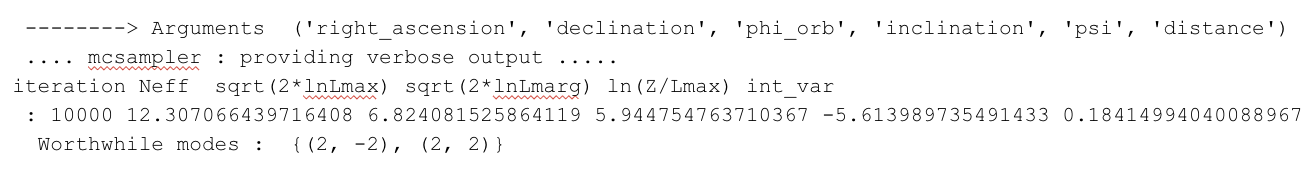
\includegraphics[width=0.9\linewidth]{output.png}
    \label{fig:output}
\end{figure}
There might be some errors about \texttt{lalym}, but you can ignore them. Finally, you can submit the job to the cluster using HTCondor and watch the progress:
\begin{minted}[frame=single,obeytabs=true,tabsize=4,linenos,numbersep=-10pt]{bash}
    condor_submit_dag -import_env master_clean.dag
    watch condor_q
\end{minted}
You always want jobs in the RUN and IDLE columns, otherwise something is wrong:
\begin{figure}[h!]
    \centering
    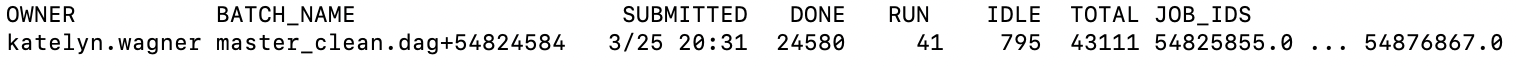
\includegraphics[width=0.75\linewidth]{condor.png}
    \label{fig:condor}
\end{figure}

Now, we have migrated to use \texttt{asimov} to automate PE using RIFT for real events. See the next tutorial folder to learn how to do this.

\end{document}
